%ex24.tex

\section{Exercice 24 - Noyau pour la 3-coloration paramétré par le vertex-cover}\label{ex16}

\subsection{Définitions}\label{ex24_def}
Soit $G = (V,E)$ un graphe. Un {\em vertex-cover} $X$ de $G$ est défini tel que :
\begin{itemize}
	\item $X \subseteq V$
	\item $\forall (x,y) \in E,\ x \in X\ ou\ y \in X$\\
\end{itemize}
De plus, on note $\Gamma_G(x)$ le voisinage du sommet $x$ dans le graphe
$G$.

\subsection{Question 1}\label{ex24_q1}
Nous voulons montrer que $G' = G \setminus X$ est un ensemble indépendant ($E' =
\emptyset$).

Par définition du $vertex-cover$ toute arête de $G$ est touchée par un des sommets de
$X$, or 
s'il existe une arête $(x,y) \in E'$, alors $x \notin X\ et\ y \notin X$.
$(x,y)$ n'est donc pas couverte par $X$,
ce qui est absurde.
Ainsi $G \setminus X$ ne contient bien aucune arête.

\subsection{Question 2}\label{ex24_q2}
Soient $x,y \in V'$ deux sommets distincts ayant le même ensemble de voisins dans $X$
$\Gamma(x) = \Gamma(y)$.
Montrons que $\chi(G \setminus \{x\}) = \chi(G)$.
Nous savons que les arêtes de $G$ sont toutes contenues dans le graphe associé à
l'ensemble de sommets $X$. Et donc une coloration valide pour $X$ est également valide
pour $G$ (en pensant à colorer les sommets de $G \setminus X$).
Puisque le voisinage de $x$ est le même que celui de $y$, nous pouvons trouver une
coloration où la couleur de $x$ est égale à celle de $y$.
Donc si nous retirons le sommet $x$, sa couleur sera toujours représentée par le
sommet $y$.
%%%%	Puisque le voisinage de $x$ est le même que celui de $y$ on peut trouver une coloration
%%%%	optimale de $V$ telle que :\\
%%%%	$\forall v \in \Gamma(x) = \Gamma(y)\\
%%%%	couleur(v) \neq couleur(x) et couleur(v) \neq couleur(y)$\\
%%%%	Nous pouvons donc attribuer la même couleur à 
\subsection{Question 3}\label{ex24_q3}

\begin{center}
\begin{algorithm}[H]
\caption{3-colorable?}\label{ex24_algo1}
\algsetup{indent=2em,linenodelimiter= }
\begin{algorithmic}[1]
\REQUIRE $G = (V,E)$
\ENSURE $G'' = (V'',E'') ; \forall x,y \in V'', \Gamma_X(x) \neq \Gamma_X(y)$
	\STATE $G'' \leftarrow G$
	\WHILE{$\exists x,y \in G''\setminus X : \Gamma_X(x) = \Gamma_X(y)$}
		\STATE $G'' \leftarrow G'' \setminus \{x\}$
	\ENDWHILE
\RETURN $G''$
\end{algorithmic}
\end{algorithm}
\end{center}

\subsubsection{(a)}\label{ex24_q3_a}

\subsubsection{(b)}\label{ex24_q3_b}
Nous allons montrer par récurence sur la taille k du vertex-cover $X$ que 
le graphe $G''$ renvoyé par l'algorithme \ref{ex24_algo1} a au
plus $k + 2^k$ sommets.

{\bfseries k = 1}\\
Pour qu'il puisse exister un vertex-cover de taille $1$, il faut qu'un sommet du graphe
$G$ soit l'extrémité de toutes ses arêtes.
Ainsi, si tel est le cas, $G$ est forcément semblable au graphe de la figure
\ref{ex24_fig1}.
Nous avons alors : 
\begin{itemize}
	\item $X = \{x\}$
	\item $G' = \{y \in V : y \neq x\}$
	\item $\forall y,y' \in G',\ \Gamma_X(y) = \Gamma_X(y')$
\end{itemize}
Et donc en appliquant l'algorithme, nous avons $V'' = \{x,y\}$, ie $|V| = 2 \leq 1 + 2^1
= 3$.

Nous supposons maintenant que cette propriété est vraie pour tout vertex-cover de taille
$k$, et nous cherchons à vérifier pour $k+1$.


% ex24_fig1.tex
\begin{figure}[h]
	\begin{center}
	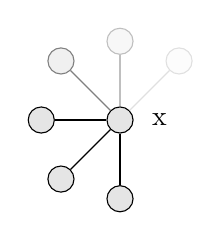
\begin{tikzpicture}
		\node[circle,draw,fill=black!10] (v) at (0,0) {};
		\node[] (vl) at (0.5,0) {x};
		\node[circle,draw,fill=black!10] (v2) at (-1,0) {}
			edge[-] (v);
		\node[circle,draw,fill=black!10] (v3) at (-0.75,-0.75) {}
			edge[-] (v);
		\node[circle,draw,fill=black!10] (v4) at (0,-1) {}
			edge[-] (v);
		\node[circle,draw=black!50,fill=black!6] (v5) at (-0.75,0.75) {}
			edge[-,draw=black!50] (v);
		\node[circle,draw=black!25,fill=black!3] (v6) at (0,1) {}
			edge[-,draw=black!25] (v);
		\node[circle,draw=black!12,fill=black!1] (v7) at (0.75,0.75) {}
			edge[-,draw=black!12] (v);
	\end{tikzpicture}
	\end{center}
	\caption{Exemple pour $k = 1$}
	\label{ex24_fig1}
\end{figure}


